\vspace{-3pt}
\section{The Tracker}\label{sec:ch3:trk}


\begin{figure}[h]
\centering
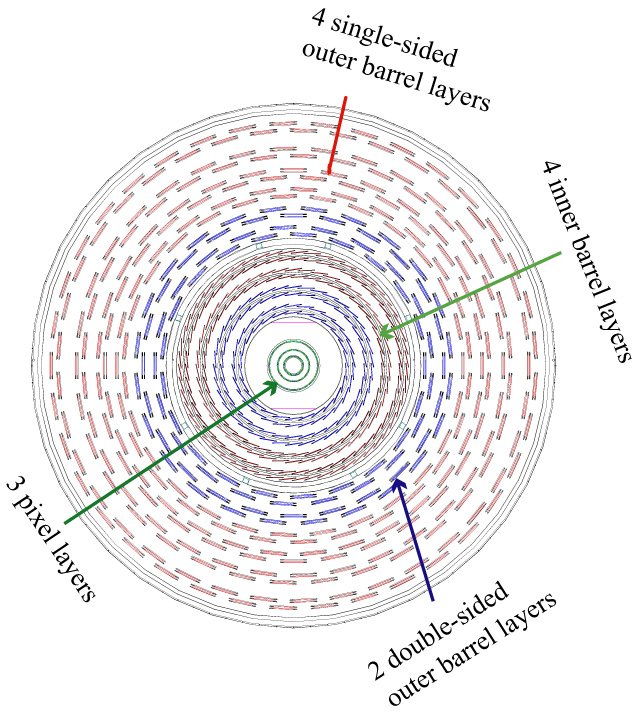
\includegraphics[width=0.5\textwidth]{figures/Barrel_0_tracker.png}
\caption{Schematic of the tracker.}
\label{fig:tracker_circular_schematic}
\end{figure}

 \begin{figure}[h]
\centering
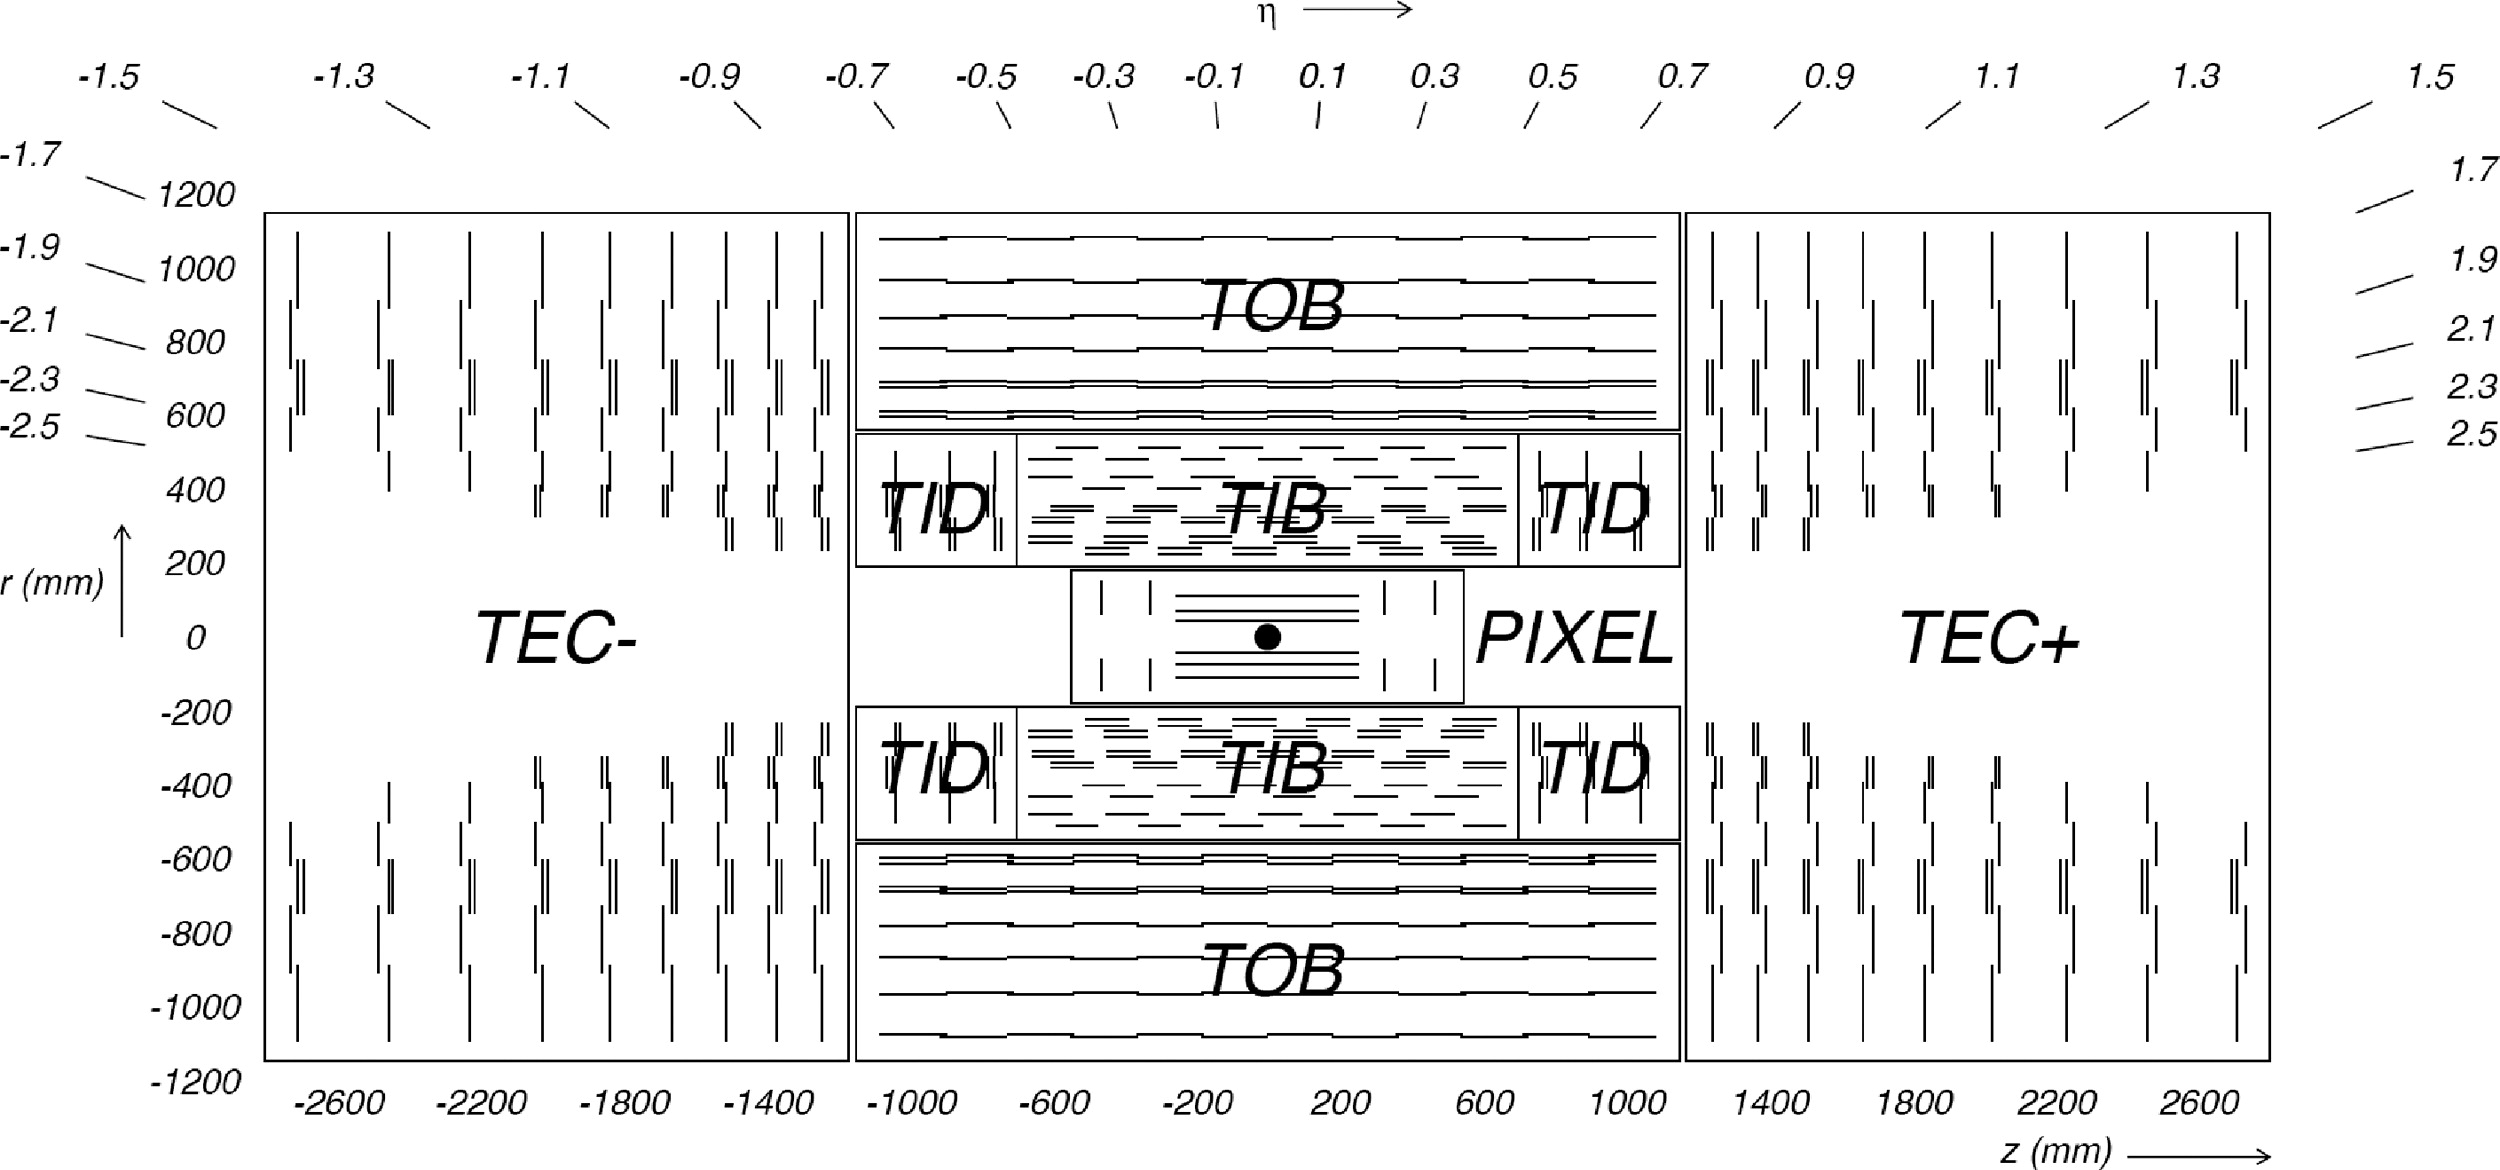
\includegraphics[width=1.0\textwidth]{figures/cms_tracker_cross_section_schematic.jpg}
\caption{Schematic of the tracker, projected onto an $z$-$r$ plane.}
\label{fig:cms_tracker_cross_section_schematic}
\end{figure}

At the innermost layer of the detector, held within the 6 meter bore of the solenoid, sits the silicon tracking system. With 1000 particles from 20 overlapping collisions bombarding the detector every 25 ns, the tracker needs a high power density system to accurately and precisely measure the tracks of individual charged particles. The high energy particles subject the electronics to high radiation levels. A radiation-hard material cooled to low temperatures is needed to withstand these high levels. For this, silicon was used, and has tracker has been operating for over a decade, longer than the planned lifetime of the detector. The tracker was built over the course of over a decade, with the input of hundreds of particle physicists from 51 institutes, including the University at Buffalo.


The tracker is composed of two subdetectors: an inner 3-layer pixel detector pixel detector and an outer 10-layer strips detector. inner , with 10 barrel layers of silicon strip tracking. In Figure~\ref{fig:tracker_circular_schematic}, the positions of these layers are shown on a circular cross-section of the cylindrical Tracker. Inside the innermost circle is the beam line where the interaction point for the detector sits. This interaction point is depicted as a black dot in Figure~\ref{fig:cms_tracker_cross_section_schematic}, which shows the detector projected onto an $r$, $z$ plane.  The 3 barrel layers of the pixel detector are the 3 lines above and below the interaction point. The pixel barrel (BPix) is 53 cm long with the largest radius at 10.2 cm, which allows coverage of $|\eta| > 2.5$. The pixel front endcaps (FPix) are position in 2 layers at $|z| = 34.5$ cm and $|z| = 46.5$ cm. The pixel layers have high granularity to allow for precise measurement of the position of the detected particles. Each pixel has an area of $100x150$ \textmu m, with 48 million pixels in BPix and 18 million in FPix~\cite{CMSExperiment}.

The strip tracker surrounds the pixel subdetector. In Figure~\ref{fig:cms_tracker_cross_section_schematic}, the subdetectors for the strips tracker are shown. The tracker inner barrel (TIB) has 4 layers with 320 \textmu m thick silicon strip sensors. The tracker outer barrel (TOB) has 6 layers with 500 \textmu m thick silicon strip sensors. The tracker has disk layers covering the high $|\eta|$ region. The tracker inner disks (TID) have 3 layers, and the tracker endcaps (TEC) have 8 layers. The TEC, TID, and FPix disk layers and the TOB, TIB, and Bpix barrel layers supply a total of 22 measurements with resolutions ranging from 23 \textmu m to 53 \textmu m, further described in Table~\ref{tab:rphi_mmts}.

\begin{figure}[h]
\centering
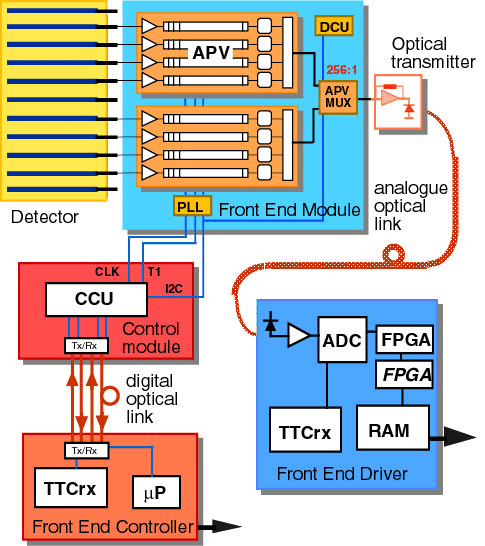
\includegraphics[width=0.5\textwidth]{figures/Read-out-scheme-of-the-CMS-Tracker.png}
\caption{Schematic of the tracker readout system~\cite{CMSExperiment}.} \label{fig:tracker_readout}
\end{figure}

\begin{table}
\begin{center}
\begin{tabular}{||c c c||} 
 \hline
 Subdetector & Resolution & $r-\phi$ Measurments \\ [0.5ex] 
 \hline\hline
 BPix/FPix &  & 3 \\ 
 \hline
 TIB/TID & 23-25 \textmu m & 4 \\
 \hline
 TOB & 35-53 \textmu m  & 6 \\
 \hline
 TEC &  & 9 \\ [1ex] 
 \hline
\end{tabular}
\caption{Resolution of the pixel and strips subdetectors with the number of measurements in $r-\phi$ each supplies~\cite{CMSExperiment}.}
\label{tab:rphi_mmts}
\end{center}
\end{table}
%
%\begin{todolist}
%	\item describe silicon strip sensors
%\end{todolist}


The tracker materials must be kept to low temperatures to mitigate the damage caused by the radiation from the beam collisions. Cooling liquid is transported to the silicon sensors by aluminum pipes, which are formed into cooling loops and attached to the sensors with aluminum ledges.

The information from the silicon sensor is sent through a readout system, shown in Figure~\ref{fig:tracker_readout}. Fiber optic cables carry analog signals from the sensors in the tracker to Front End Drivers (FEDs). The FEDs convert the analog signals to digital. Front End Controllers (FECs) transmit signals from the clock, control systems, and trigger. The information from the tracker is vital to the high level trigger (HLT) decisions, which reduce the rate of incoming collisions data by a factor of 400. Silicon modules contain either one of the 320 \textmu m or 2 of the 500 \textmu m thick silicon sensors. The modules are grouped into power groups that are each powered by one power supply, which supplies 2 low voltage lines at 1.25 V and 2.5 V, and 2 high voltage lines. The silicon sensors are made of p-on-n type material. On the back, n type aluminum is used to connect to a positive voltage. On the other side are the p+ type silicon strip diodes. 

The Detector Control Systems (DCS) are designed using a Supervising Control and Data Acquisition (SCADA) program developed with WinCCOA. The DCS is a Final State Machine tree that controls all of the power supplies. A Detector Control Unit monitors the low voltage, leakage current, and temperature of the silicon sensors.

The radiation length of materials used in the tracker shown in Figure~\ref{fig:tracker_radiation_length.}.

\begin{figure}[h]
\centering
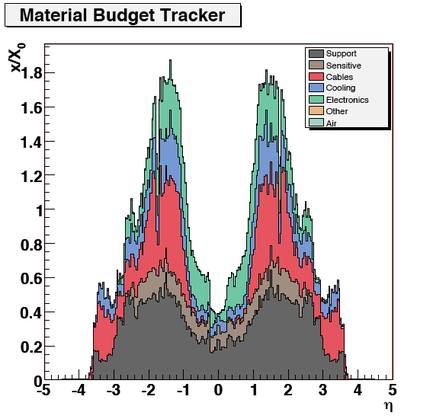
\includegraphics[width=0.5\textwidth]{figures/tracker_radiation_length_XoverX0.png}
\caption{Radiation length of materials used in the tracker~\cite{CMSExperiment}.}
\label{fig:tracker_radiation_length.}
\end{figure}


